% ==============================================================================
% BỘ ĐỀ THAM KHẢO TUYỂN SINH 10 NĂM HỌC 2026-2027 SỞ GD&ĐT TP.HCM
% ĐỢT 10: CỤM 7 - ĐỀ 2 & CỤM 7 - ĐỀ 3 (14 CÂU TỰ LUẬN)
% ==============================================================================

% ==============================================================================
% CỤM 7 - ĐỀ THAM KHẢO 2 (Đề số 20)
% ==============================================================================

\begin{bt}%[9D6H18-2]
% nguon: Đề tham khảo Tuyển sinh 10 năm học 2026-2027 Sở GD&ĐT TP.HCM - Cụm 7 Đề 2, Bài 1
	Cho parabol $(P)\colon y = 2x^2$.
	\begin{enumerate}[a)]
		\item Vẽ đồ thị $(P)$ của hàm số trên.
		\item Tìm những điểm $M$ thuộc $(P)$ thỏa mãn điều kiện tung độ lớn hơn hoành độ $1$ đơn vị.
	\end{enumerate}
	\loigiai{
		\begin{enumerate}[a)]
			\item Bảng giá trị tương ứng giữa $x$ và $y$ của parabol $(P)\colon y = 2x^2$:
			\begin{center}
				\begin{tabular}{|c|c|c|c|c|c|}
					\hline
					$x$ & $-2$ & $-1$ & $0$ & $1$ & $2$ \\
					\hline
					$y = 2x^2$ & $8$ & $2$ & $0$ & $2$ & $8$ \\
					\hline
				\end{tabular}
			\end{center}
			Đồ thị $(P)$ là một parabol đi qua gốc tọa độ $O(0;0)$, nằm phía trên trục hoành và nhận trục tung $Oy$ làm trục đối xứng.
			\begin{center}
				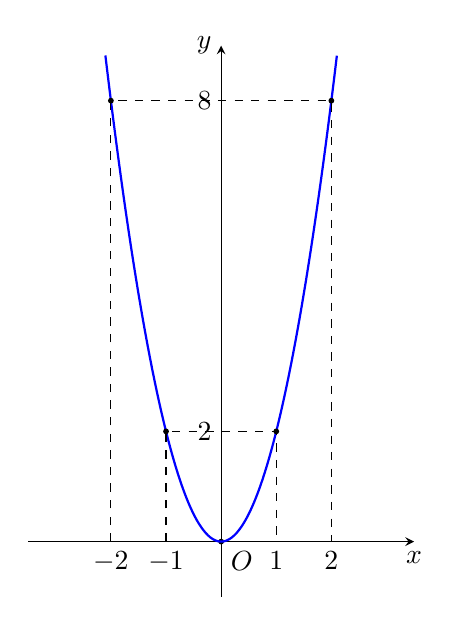
\begin{tikzpicture}[>=stealth, scale=0.7]
					\draw[->] (-3.5,0) -- (3.5,0) node[below] {$x$};
					\draw[->] (0,-1) -- (0,9) node[left] {$y$};
					\fill (0,0) circle (1.5pt) node[below right] {$O$};
					\draw[smooth, samples=100, domain=-2.1:2.1, thick, color=blue] plot(\x, {2*(\x)^2});
					\draw[dashed] (-2,0) node[below] {$-2$} -- (-2,8) -- (0,8) node[left] {$8$} -- (2,8) -- (2,0) node[below] {$2$};
					\draw[dashed] (-1,0) node[below] {$-1$} -- (-1,2) -- (0,2) node[left] {$2$} -- (1,2) -- (1,0) node[below] {$1$};
					\fill (-2,8) circle (1.5pt) (2,8) circle (1.5pt) (-1,2) circle (1.5pt) (1,2) circle (1.5pt);
				\end{tikzpicture}
			\end{center}
			\item Vì điểm cần tìm có tung độ lớn hơn hoành độ $1$ đơn vị nên ta có $y = x + 1$.
			
			Mặt khác điểm đó thuộc $(P)$ nên ta có phương trình:
			$$2x^2 = x + 1 \iff 2x^2 - x - 1 = 0.$$
			Phương trình có các hệ số $a = 2, b = -1, c = -1$ với $a + b + c = 0$ nên có hai nghiệm:
			$$x_1 = 1,\quad x_2 = -\dfrac{1}{2}.$$
			- Với $x_1 = 1 \implies y_1 = 1 + 1 = 2$.
			
			- Với $x_2 = -\dfrac{1}{2} \implies y_2 = -\dfrac{1}{2} + 1 = \dfrac{1}{2}$.
			
			Vậy tọa độ các điểm cần tìm là $(1; 2)$ và $\left(-\dfrac{1}{2}; \dfrac{1}{2}\right)$.
		\end{enumerate}
	}
\end{bt}

\begin{bt}%[9D6H20-2]
% nguon: Đề tham khảo Tuyển sinh 10 năm học 2026-2027 Sở GD&ĐT TP.HCM - Cụm 7 Đề 2, Bài 2
	Cho phương trình $3x^2 - 7x + 3 = 0$.
	\begin{enumerate}[a)]
		\item Chứng minh phương trình luôn có hai nghiệm phân biệt $x_1, x_2$.
		\item Không giải phương trình, hãy tính giá trị của biểu thức:
		$$A = \dfrac{18x_2}{5x_1 - x_2 + \dfrac{7}{3}} + \dfrac{18x_1}{5x_2 - x_1 + \dfrac{7}{3}}.$$
	\end{enumerate}
	\loigiai{
		\begin{enumerate}[a)]
			\item Phương trình $3x^2 - 7x + 3 = 0$ có $a = 3, b = -7, c = 3$.
			
			Ta có:
			$$\Delta = b^2 - 4ac = (-7)^2 - 4 \cdot 3 \cdot 3 = 49 - 36 = 13 > 0.$$
			Vì $\Delta > 0$ nên phương trình luôn có hai nghiệm phân biệt $x_1, x_2$.
			\item Theo định lí Viète, ta có:
			$$\begin{cases} x_1 + x_2 = \dfrac{7}{3} \\ x_1 x_2 = 1. \end{cases}$$
			Ta có:
			$$x_1^2 + x_2^2 = (x_1 + x_2)^2 - 2x_1 x_2 = \left(\dfrac{7}{3}\right)^2 - 2 \cdot 1 = \dfrac{49}{9} - 2 = \dfrac{31}{9}.$$
			Thay $\dfrac{7}{3} = x_1 + x_2$ vào các mẫu thức của biểu thức $A$, ta được:
			$$5x_1 - x_2 + \dfrac{7}{3} = 5x_1 - x_2 + (x_1 + x_2) = 6x_1;$$
			$$5x_2 - x_1 + \dfrac{7}{3} = 5x_2 - x_1 + (x_1 + x_2) = 6x_2.$$
			Khi đó biểu thức $A$ trở thành:
			$$A = \dfrac{18x_2}{6x_1} + \dfrac{18x_1}{6x_2} = \dfrac{3x_2}{x_1} + \dfrac{3x_1}{x_2} = \dfrac{3(x_1^2 + x_2^2)}{x_1 x_2}.$$
			Thay số vào, ta được:
			$$A = \dfrac{3 \cdot \dfrac{31}{9}}{1} = \dfrac{31}{3}.$$
			Vậy $A = \dfrac{31}{3}$.
		\end{enumerate}
	}
\end{bt}

\begin{bt}%[9D8H26-3]
% nguon: Đề tham khảo Tuyển sinh 10 năm học 2026-2027 Sở GD&ĐT TP.HCM - Cụm 7 Đề 2, Bài 3
	Phổ điểm kiểm tra môn Toán cuối kì 2 của $53$ học sinh lớp 9A được thống kê trong bảng sau:
	\begin{center}
		\begin{tabular}{|l|c|c|c|c|c|c|c|c|c|c|c|}
			\hline
			\textbf{Điểm số} & 5{,}0 & 5{,}5 & 6{,}0 & 6{,}5 & 7{,}0 & 7{,}5 & 8{,}0 & 8{,}5 & 9{,}0 & 9{,}5 & 10 \\
			\hline
			\textbf{Số học sinh} & 4 & 10 & 15 & 8 & 7 & 3 & 2 & 1 & 1 & 1 & 1 \\
			\hline
		\end{tabular}
	\end{center}
	\begin{enumerate}[a)]
		\item Tính điểm trung bình cộng môn Toán của lớp 9A.
		\item Tính xác suất thực nghiệm của biến cố $A$: ``Học sinh được chọn có điểm số là $6{,}5$ điểm''.
		\item Tính xác suất thực nghiệm của biến cố $B$: ``Học sinh được chọn có điểm số đạt loại giỏi (từ $8{,}0$ điểm trở lên)''.
	\end{enumerate}
	\loigiai{
		Tổng số học sinh lớp 9A là $n(\Omega) = 53$.
		\begin{enumerate}[a)]
			\item Tổng số điểm của cả lớp là:
			$$S = 5 \cdot 4 + 5{,}5 \cdot 10 + 6 \cdot 15 + 6{,}5 \cdot 8 + 7 \cdot 7 + 7{,}5 \cdot 3 + 8 \cdot 2 + 8{,}5 \cdot 1 + 9 \cdot 1 + 9{,}5 \cdot 1 + 10 \cdot 1 = 341{,}5.$$
			Điểm trung bình cộng của lớp 9A là:
			$$\overline{X} = \dfrac{341{,}5}{53} = \dfrac{683}{106} \approx 6{,}44.$$
			\item Số học sinh đạt điểm $6{,}5$ là $8$ học sinh, nên $n(A) = 8$.
			
			Xác suất thực nghiệm của biến cố $A$ là:
			$$P(A) = \dfrac{n(A)}{n(\Omega)} = \dfrac{8}{53}.$$
			\item Các điểm giỏi từ $8{,}0$ điểm trở lên gồm $8{,}0; 8{,}5; 9{,}0; 9{,}5; 10$.
			
			Số học sinh đạt loại giỏi là:
			$$n(B) = 2 + 1 + 1 + 1 + 1 = 6\text{ (học sinh)}.$$
			Xác suất thực nghiệm của biến cố $B$ là:
			$$P(B) = \dfrac{n(B)}{n(\Omega)} = \dfrac{6}{53}.$$
		\end{enumerate}
	}
\end{bt}

\begin{bt}%[9D6V21-3]
% nguon: Đề tham khảo Tuyển sinh 10 năm học 2026-2027 Sở GD&ĐT TP.HCM - Cụm 7 Đề 2, Bài 4
	Từ một khối gỗ hình hộp chữ nhật có kích thước chiều dài, chiều rộng và chiều cao lần lượt là $x + 5$; $x + 2$ và $x$ (mét), người ta khoét đi một lỗ có dạng hình lập phương cạnh là $x - 1$ (mét) ($x > 1$).
	\begin{enumerate}[a)]
		\item Viết biểu thức thu gọn $A$ biểu thị phần thể tích còn lại của khối gỗ theo $x$.
		\item Biết thể tích còn lại của khối gỗ là $7\text{ m}^3$, hãy tìm giá trị của $x$.
	\end{enumerate}
	\loigiai{
		\begin{enumerate}[a)]
			\item Thể tích khối gỗ hình hộp chữ nhật ban đầu là:
			$$V_1 = x(x + 5)(x + 2) = x(x^2 + 7x + 10) = x^3 + 7x^2 + 10x\text{ (m}^3).$$
			Thể tích phần lỗ khoét hình lập phương là:
			$$V_2 = (x - 1)^3 = x^3 - 3x^2 + 3x - 1\text{ (m}^3).$$
			Biểu thức $A$ biểu thị phần thể tích còn lại của khối gỗ là:
			$$A = V_1 - V_2 = (x^3 + 7x^2 + 10x) - (x^3 - 3x^2 + 3x - 1) = 10x^2 + 7x + 1\text{ (m}^3).$$
			\item Theo đề bài thể tích còn lại là $7\text{ m}^3$ nên ta có phương trình:
			$$10x^2 + 7x + 1 = 7 \iff 10x^2 + 7x - 6 = 0.$$
			Ta có $\Delta = 7^2 - 4 \cdot 10 \cdot (-6) = 49 + 240 = 289 = 17^2 > 0$.
			
			Phương trình có hai nghiệm:
			$$x_1 = \dfrac{-7 + 17}{20} = 0{,}5,\quad x_2 = \dfrac{-7 - 17}{20} = -1{,}2.$$
			Vì cạnh hình lập phương là $x - 1 > 0 \implies x > 1$, nên cả hai giá trị $x_1 = 0{,}5$ và $x_2 = -1{,}2$ đều không thỏa mãn điều kiện.
			
			Vậy không có giá trị nào của $x$ thỏa mãn yêu cầu đề bài.
		\end{enumerate}
	}
\end{bt}

\begin{bt}%[9H0V31-3]
% nguon: Đề tham khảo Tuyển sinh 10 năm học 2026-2027 Sở GD&ĐT TP.HCM - Cụm 7 Đề 2, Bài 5
	Một khối hộp chữ nhật đặc ruột bằng sắt có ba kích thước là $12\text{ cm}$, $10\text{ cm}$, $7\text{ cm}$ bị khoét bởi một nửa hình trụ có đường kính $4\text{ cm}$ và chiều dài $12\text{ cm}$.
	\begin{enumerate}[a)]
		\item Tính thể tích khối kim loại còn lại (kết quả làm tròn đến hàng đơn vị của $\text{cm}^3$).
		\item Người ta nấu nóng chảy toàn bộ phần kim loại còn lại này để đúc các viên bi sắt hình cầu có bán kính $1\text{ cm}$. Hỏi đúc được nhiều nhất bao nhiêu viên bi sắt như thế?
	\end{enumerate}
	\loigiai{
		\begin{enumerate}[a)]
			\item Thể tích của khối hộp chữ nhật ban đầu là:
			$$V_1 = 12 \cdot 10 \cdot 7 = 840\text{ (cm}^3).$$
			Bán kính đáy của nửa hình trụ bị khoét là:
			$$R = \dfrac{4}{2} = 2\text{ (cm)}.$$
			Thể tích phần nửa hình trụ bị khoét đi là:
			$$V_2 = \dfrac{1}{2} \cdot \pi R^2 h = \dfrac{1}{2} \cdot \pi \cdot 2^2 \cdot 12 = 24\pi\text{ (cm}^3).$$
			Thể tích của khối kim loại còn lại là:
			$$V = V_1 - V_2 = 840 - 24\pi \approx 764{,}6 \approx 765\text{ (cm}^3).$$
			\item Thể tích của một viên bi sắt hình cầu bán kính $r = 1\text{ cm}$ là:
			$$V_{\text{bi}} = \dfrac{4}{3}\pi r^3 = \dfrac{4}{3}\pi \cdot 1^3 = \dfrac{4}{3}\pi\text{ (cm}^3).$$
			Số viên bi sắt đúc được nhiều nhất là:
			$$n = \dfrac{V}{V_{\text{bi}}} = \dfrac{840 - 24\pi}{\dfrac{4}{3}\pi} \approx 182{,}54.$$
			Vì số viên bi phải là số nguyên nên có thể đúc được nhiều nhất $182$ viên bi.
		\end{enumerate}
	}
\end{bt}

\begin{bt}%[9D1H3-4]
% nguon: Đề tham khảo Tuyển sinh 10 năm học 2026-2027 Sở GD&ĐT TP.HCM - Cụm 7 Đề 2, Bài 6
	Có hai chiếc thùng, thùng thứ nhất đang chứa $95$ lít dầu, thùng thứ hai đang chứa $80$ lít dầu. Người ta lấy bớt dầu ở cả hai thùng. Nếu thùng thứ nhất lấy ra ít hơn thùng thứ hai $5$ lít dầu thì khi đó hai lần số dầu còn lại ở thùng thứ hai nhiều hơn số dầu còn lại ở thùng thứ nhất là $40$ lít. Hỏi sau khi lấy ra, số dầu còn lại ở thùng thứ hai là bao nhiêu lít?
	\loigiai{
		Gọi $x$ (lít) là số lít dầu lấy ra từ thùng thứ nhất ($0 < x < 95$).
		
		Gọi $y$ (lít) là số lít dầu lấy ra từ thùng thứ hai ($5 < y < 80$).
		
		Số lít dầu còn lại ở thùng thứ nhất là:
		$$95 - x\text{ (lít)}.$$
		Số lít dầu còn lại ở thùng thứ hai là:
		$$80 - y\text{ (lít)}.$$
		Vì thùng thứ nhất lấy ra ít hơn thùng thứ hai $5$ lít dầu nên ta có phương trình:
		$$y - x = 5. \quad (1)$$
		Vì hai lần số dầu còn lại ở thùng thứ hai nhiều hơn số dầu còn lại ở thùng thứ nhất là $40$ lít nên ta có phương trình:
		$$2(80 - y) - (95 - x) = 40 \iff 160 - 2y - 95 + x = 40 \iff x - 2y = -25. \quad (2)$$
		Từ $(1)$ và $(2)$, ta có hệ phương trình:
		$$\begin{cases} y - x = 5 \\ x - 2y = -25 \end{cases} \iff \begin{cases} -x + y = 5 \\ x - 2y = -25 \end{cases} \iff \begin{cases} -y = -20 \\ x = y - 5 \end{cases} \iff \begin{cases} y = 20\text{ (thỏa mãn)} \\ x = 15\text{ (thỏa mãn)}. \end{cases}$$
		Số lít dầu còn lại ở thùng thứ hai là:
		$$80 - 20 = 60\text{ (lít)}.$$
		Vậy sau khi lấy ra, thùng thứ hai còn lại $60$ lít dầu.
	}
\end{bt}

\begin{bt}%[9H9C29-3]
% nguon: Đề tham khảo Tuyển sinh 10 năm học 2026-2027 Sở GD&ĐT TP.HCM - Cụm 7 Đề 2, Bài 7
	Từ điểm $A$ nằm ngoài đường tròn $(O; R)$, kẻ hai tiếp tuyến $AB, AC$ đến $(O)$ ($B, C$ là hai tiếp điểm). Gọi $H$ là giao điểm của $OA$ và $BC$.
	\begin{enumerate}[a)]
		\item Chứng minh $OA$ là đường trung trực của đoạn thẳng $BC$ và tứ giác $OBAC$ là tứ giác nội tiếp.
		\item Chứng minh $R = \dfrac{(AB + AC) \cdot OH}{BC}$.
		\item Trên đoạn $AH$ lấy điểm $D$ sao cho $HB = HD$. Qua $D$ kẻ đường thẳng vuông góc với $OA$ cắt $AB$ tại $E$. Gọi $I$ là trung điểm của đoạn thẳng $OE$. Cho $R = 5\text{ cm}$, hãy tính số đo của góc $\widehat{BHI}$ và độ dài cạnh $BE$.
	\end{enumerate}
	\loigiai{
		\begin{center}
			\begin{tikzpicture}[>=stealth, scale=0.9]
				\coordinate (O) at (0,0);
				\def\r{2.5}
				\draw (O) circle (\r);
				\coordinate (A) at (5,0);
				\pgfmathsetmacro{\distA}{5}
				\pgfmathsetmacro{\alphaA}{acos(\r/\distA)}
				\coordinate (B) at ({\alphaA}:\r);
				\coordinate (C) at ({-\alphaA}:\r);
				\draw (A) -- (B);
				\draw (A) -- (C);
				\draw (O) -- (B);
				\draw (O) -- (C);
				\draw (O) -- (A);
				\draw (B) -- (C);
				\coordinate (H) at (intersection of O--A and B--C);
				% D thuộc AH sao cho HD = HB
				% H có tọa độ xH = r*cos(alpha) = 2.5*0.5 = 1.25. HB = r*sin(60) = 2.5*sqrt(3)/2 ~ 2.165
				% A ở (5,0), H ở (1.25,0), D ở (1.25 + 2.165, 0) = (3.415, 0)
				\pgfmathsetmacro{\hbVal}{\r*sin(\alphaA)}
				\coordinate (D) at ($(H)+(\hbVal,0)$);
				% DE vuông góc OA => đường thẳng thẳng đứng qua D, cắt AB tại E
				\coordinate (E) at (intersection of D--+(0,3) and A--B);
				\draw (D) -- (E);
				\draw (O) -- (E);
				\coordinate (I) at ($(O)!0.5!(E)$);
				\draw (H) -- (I);
				\node at (O) [left] {$O$};
				\node at (A) [right] {$A$};
				\node at (B) [above] {$B$};
				\node at (C) [below] {$C$};
				\node at (H) [below left] {$H$};
				\node at (D) [below] {$D$};
				\node at (E) [above] {$E$};
				\node at (I) [above left] {$I$};
				\fill (O) circle (1.5pt) (A) circle (1.5pt) (B) circle (1.5pt) (C) circle (1.5pt) (H) circle (1.5pt) (D) circle (1.5pt) (E) circle (1.5pt) (I) circle (1.5pt);
			\end{tikzpicture}
		\end{center}
		\begin{enumerate}[a)]
			\item Vì $AB, AC$ là hai tiếp tuyến của $(O)$ nên $AB = AC$ và $\widehat{ABO} = \widehat{ACO} = 90^\circ$.
			
			Lại có $OB = OC = R$ nên $OA$ là đường trung trực của đoạn thẳng $BC$, suy ra $OA \perp BC$ tại $H$.
			
			Tứ giác $OBAC$ có $\widehat{ABO} + \widehat{ACO} = 90^\circ + 90^\circ = 180^\circ$, do đó $OBAC$ là tứ giác nội tiếp đường tròn đường kính $OA$.
			\item Vì $OA$ là đường trung trực của $BC$ nên $H$ là trung điểm của $BC \implies BC = 2BH$.
			
			Xét tam giác vuông $OBA$ tại $B$ có đường cao $BH$, theo hệ thức lượng trong tam giác vuông hoặc tam giác đồng dạng ($\Delta OHB \backsim \Delta OBA$):
			$$\dfrac{OH}{OB} = \dfrac{BH}{AB} \implies OH \cdot AB = OB \cdot BH \iff R \cdot BH = AB \cdot OH \iff R = \dfrac{AB \cdot OH}{BH}.$$
			Nhân cả tử và mẫu với $2$, ta có:
			$$R = \dfrac{2AB \cdot OH}{2BH} = \dfrac{(AB + AB) \cdot OH}{BC}.$$
			Vì $AB = AC$ nên ta suy ra:
			$$R = \dfrac{(AB + AC) \cdot OH}{BC}.$$
			\item Xét tam giác vuông $OBE$ tại $B$ có $I$ là trung điểm của cạnh huyền $OE \implies IB = \dfrac{1}{2}OE$.
			
			Tam giác $ODE$ vuông tại $D$ (do $DE \perp OA$) có $I$ là trung điểm cạnh huyền $OE \implies ID = \dfrac{1}{2}OE$.
			
			Suy ra $IB = ID$.
			
			Xét $\Delta HBI$ và $\Delta HDI$ có:
			$$HB = HD\text{ (giả thiết)},\quad HI\text{ chung},\quad IB = ID.$$
			Do đó $\Delta HBI = \Delta HDI\text{ (c-c-c)} \implies \widehat{BHI} = \widehat{DHI}$.
			
			Suy ra $HI$ là tia phân giác của $\widehat{BHD}$.
			
			Vì $OA \perp BC$ nên $\widehat{BHD} = 90^\circ \implies \widehat{BHI} = \dfrac{90^\circ}{2} = 45^\circ$.
			
			Mặt khác, $\Delta HBD$ vuông cân tại $H$ (vì $HB = HD$ và $\widehat{BHD} = 90^\circ$) nên $\widehat{HDB} = 45^\circ$.
			
			Tứ giác $OBED$ có $\widehat{OBE} = \widehat{ODE} = 90^\circ$ nên là tứ giác nội tiếp đường tròn đường kính $OE$.
			
			Suy ra $\widehat{OEB} = \widehat{ODB} = \widehat{HDB} = 45^\circ$ (cùng chắn cung $OB$).
			
			Do đó tam giác $OBE$ vuông cân tại $B$, suy ra $BE = OB = R = 5\text{ cm}$.
			
			Vậy $\widehat{BHI} = 45^\circ$ và $BE = 5\text{ cm}$.
		\end{enumerate}
	}
\end{bt}

% ==============================================================================
% CỤM 7 - ĐỀ THAM KHẢO 3 (Đề số 21)
% ==============================================================================

\begin{bt}%[9D6H18-2]
% nguon: Đề tham khảo Tuyển sinh 10 năm học 2026-2027 Sở GD&ĐT TP.HCM - Cụm 7 Đề 3, Bài 1
	Cho hàm số $y = -\dfrac{1}{4}x^2$ có đồ thị là parabol $(P)$.
	\begin{enumerate}[a)]
		\item Vẽ đồ thị $(P)$ của hàm số trên mặt phẳng tọa độ $Oxy$.
		\item Tìm những điểm $M$ thuộc $(P)$ có tung độ gấp $4$ lần hoành độ.
	\end{enumerate}
	\loigiai{
		\begin{enumerate}[a)]
			\item Bảng giá trị của hàm số $y = -\dfrac{1}{4}x^2$:
			\begin{center}
				\begin{tabular}{|c|c|c|c|c|c|}
					\hline
					$x$ & $-4$ & $-2$ & $0$ & $2$ & $4$ \\
					\hline
					$y = -\dfrac{1}{4}x^2$ & $-4$ & $-1$ & $0$ & $-1$ & $-4$ \\
					\hline
				\end{tabular}
			\end{center}
			Đồ thị $(P)$ là một parabol đi qua gốc tọa độ $O(0;0)$, nằm phía dưới trục hoành và nhận trục tung $Oy$ làm trục đối xứng.
			\begin{center}
				\begin{tikzpicture}[>=stealth, scale=0.7]
					\draw[->] (-5,0) -- (5,0) node[below] {$x$};
					\draw[->] (0,-5) -- (0,1.5) node[left] {$y$};
					\fill (0,0) circle (1.5pt) node[above right] {$O$};
					\draw[smooth, samples=100, domain=-4.2:4.2, thick, color=blue] plot(\x, {-1/4*(\x)^2});
					\draw[dashed] (-4,0) node[above] {$-4$} -- (-4,-4) -- (0,-4) node[right] {$-4$} -- (4,-4) -- (4,0) node[above] {$4$};
					\draw[dashed] (-2,0) node[above] {$-2$} -- (-2,-1) -- (0,-1) node[right] {$-1$} -- (2,-1) -- (2,0) node[above] {$2$};
					\fill (-4,-4) circle (1.5pt) (4,-4) circle (1.5pt) (-2,-1) circle (1.5pt) (2,-1) circle (1.5pt);
				\end{tikzpicture}
			\end{center}
			\item Vì tung độ gấp $4$ lần hoành độ nên ta có phương trình:
			$$y = 4x.$$
			Mặt khác điểm đó thuộc $(P)$ nên:
			$$-\dfrac{1}{4}x^2 = 4x \iff \dfrac{1}{4}x^2 + 4x = 0 \iff x\left(\dfrac{1}{4}x + 4\right) = 0 \iff \left[\begin{aligned} &x = 0 \\ &x = -16. \end{aligned}\right.$$
			- Với $x = 0 \implies y = 0$.
			
			- Với $x = -16 \implies y = 4 \cdot (-16) = -64$.
			
			Vậy tọa độ các điểm cần tìm là $(0; 0)$ và $(-16; -64)$.
		\end{enumerate}
	}
\end{bt}

\begin{bt}%[9D6H20-2]
% nguon: Đề tham khảo Tuyển sinh 10 năm học 2026-2027 Sở GD&ĐT TP.HCM - Cụm 7 Đề 3, Bài 2
	Cho phương trình $2x^2 - x - 4 = 0$.
	\begin{enumerate}[a)]
		\item Chứng minh phương trình luôn có hai nghiệm phân biệt $x_1, x_2$.
		\item Không giải phương trình, hãy tính giá trị của biểu thức:
		$$A = \dfrac{x_1 + 2\,026}{x_2} + \dfrac{x_2 + 2\,026}{x_1}.$$
	\end{enumerate}
	\loigiai{
		\begin{enumerate}[a)]
			\item Phương trình $2x^2 - x - 4 = 0$ có $a = 2, b = -1, c = -4$.
			
			Vì $a \cdot c = 2 \cdot (-4) = -8 < 0$ nên phương trình luôn có hai nghiệm phân biệt $x_1, x_2$.
			\item Theo định lí Viète, ta có:
			$$\begin{cases} x_1 + x_2 = -\dfrac{b}{a} = \dfrac{1}{2} \\ x_1 x_2 = \dfrac{c}{a} = -2. \end{cases}$$
			Ta có:
			$$x_1^2 + x_2^2 = (x_1 + x_2)^2 - 2x_1 x_2 = \left(\dfrac{1}{2}\right)^2 - 2 \cdot (-2) = \dfrac{1}{4} + 4 = \dfrac{17}{4}.$$
			Quy đồng mẫu số biểu thức $A$:
			$$A = \dfrac{x_1(x_1 + 2\,026) + x_2(x_2 + 2\,026)}{x_1 x_2} = \dfrac{(x_1^2 + x_2^2) + 2\,026(x_1 + x_2)}{x_1 x_2}.$$
			Thay các giá trị vào biểu thức $A$, ta được:
			$$A = \dfrac{\dfrac{17}{4} + 2\,026 \cdot \dfrac{1}{2}}{-2} = \dfrac{\dfrac{17}{4} + 1\,013}{-2} = \dfrac{\dfrac{4\,069}{4}}{-2} = -\dfrac{4\,069}{8}.$$
			Vậy $A = -\dfrac{4\,069}{8}$.
		\end{enumerate}
	}
\end{bt}

\begin{bt}%[9D8H26-3]
% nguon: Đề tham khảo Tuyển sinh 10 năm học 2026-2027 Sở GD&ĐT TP.HCM - Cụm 7 Đề 3, Bài 3
	Biểu đồ hình quạt tròn biểu diễn kết quả điểm kiểm tra thường xuyên lần hai môn Toán của $40$ học sinh lớp 9A có tỉ lệ: Điểm $6$ chiếm $15\%$, Điểm $7$ chiếm $20\%$, Điểm $8$ chiếm $25\%$, Điểm $9$ chiếm $30\%$, Điểm $10$ chiếm $10\%$.
	\begin{enumerate}[a)]
		\item Tính tổng số học sinh đạt điểm $8$ và điểm $9$.
		\item Chọn ngẫu nhiên một bạn trong lớp. Tính xác suất của biến cố: ``Bạn được chọn có điểm kiểm tra Toán thấp nhất là $8$ điểm''.
	\end{enumerate}
	\loigiai{
		\begin{enumerate}[a)]
			\item Tỉ lệ phần trăm học sinh đạt điểm $8$ và điểm $9$ là:
			$$25\% + 30\% = 55\%.$$
			Tổng số học sinh đạt điểm $8$ và điểm $9$ là:
			$$40 \cdot 55\% = 22\text{ (học sinh)}.$$
			\item Số học sinh trong không gian mẫu là $n(\Omega) = 40$.
			
			Học sinh có điểm kiểm tra Toán thấp nhất là $8$ điểm gồm các bạn đạt điểm $8$, điểm $9$ hoặc điểm $10$.
			
			Tỉ lệ phần trăm các bạn có điểm kiểm tra từ $8$ điểm trở lên là:
			$$25\% + 30\% + 10\% = 65\%.$$
			Số học sinh có điểm kiểm tra đạt ít nhất $8$ điểm là:
			$$n(A) = 40 \cdot 65\% = 26\text{ (học sinh)}.$$
			Xác suất của biến cố cần tìm là:
			$$P(A) = \dfrac{n(A)}{n(\Omega)} = \dfrac{26}{40} = \dfrac{13}{20} = 0{,}65.$$
		\end{enumerate}
	}
\end{bt}

\begin{bt}%[9D6V21-3]
% nguon: Đề tham khảo Tuyển sinh 10 năm học 2026-2027 Sở GD&ĐT TP.HCM - Cụm 7 Đề 3, Bài 4
	Một mảnh đất hình chữ nhật có chiều dài $30\text{ m}$ và chiều rộng $20\text{ m}$. Người ta làm một lối đi xung quanh ba cạnh của mảnh đất có cùng bề rộng là $x\text{ (m)}$ ($0 < x < 10$), gồm một cạnh chiều rộng và hai cạnh chiều dài.
	\begin{enumerate}[a)]
		\item Viết biểu thức thu gọn $S$ biểu diễn diện tích lối đi theo $x$.
		\item Biết diện tích phần đất còn lại sau khi làm lối đi là $448\text{ m}^2$, hãy tìm giá trị của $x$.
	\end{enumerate}
	\loigiai{
		\begin{enumerate}[a)]
			\item Chiều dài của phần đất còn lại là:
			$$30 - x\text{ (m)}.$$
			Chiều rộng của phần đất còn lại là:
			$$20 - 2x\text{ (m)}.$$
			Diện tích của mảnh đất ban đầu là:
			$$30 \cdot 20 = 600\text{ (m}^2).$$
			Diện tích phần đất còn lại là:
			$$(30 - x)(20 - 2x) = 600 - 60x - 20x + 2x^2 = 2x^2 - 80x + 600\text{ (m}^2).$$
			Biểu thức $S$ biểu diễn diện tích của lối đi là:
			$$S = 600 - (2x^2 - 80x + 600) = -2x^2 + 80x\text{ (m}^2).$$
			\item Theo đề bài, diện tích phần đất còn lại là $448\text{ m}^2$ nên ta có phương trình:
			$$2x^2 - 80x + 600 = 448 \iff 2x^2 - 80x + 152 = 0 \iff x^2 - 40x + 76 = 0.$$
			Ta có $\Delta' = (-20)^2 - 1 \cdot 76 = 400 - 76 = 324 = 18^2 > 0$.
			
			Phương trình có hai nghiệm:
			$$x_1 = 20 - 18 = 2\text{ (thỏa mãn } 0 < x < 10),\quad x_2 = 20 + 18 = 38\text{ (loại)}.$$
			Vậy bề rộng lối đi là $x = 2\text{ m}$.
		\end{enumerate}
	}
\end{bt}

\begin{bt}%[9H0V31-3]
% nguon: Đề tham khảo Tuyển sinh 10 năm học 2026-2027 Sở GD&ĐT TP.HCM - Cụm 7 Đề 3, Bài 5
	Người ta đổ một lượng nước vào một chiếc phễu thủy tinh hình nón có chiều cao $20\text{ cm}$ và bán kính miệng đáy là $R$. Chiều cao của cột nước bên trong phễu là $10\text{ cm}$ (đỉnh phễu hướng xuống dưới).
	\begin{enumerate}[a)]
		\item Tính thể tích của lượng nước trong phễu và thể tích phần phễu không chứa nước theo $R$.
		\item Bịt kín miệng phễu và lật ngược phễu lại (đỉnh phễu hướng lên trên). Chiều cao của cột nước trong phễu lúc này là bao nhiêu? (kết quả làm tròn đến hàng phần chục của $\text{cm}$).
	\end{enumerate}
	\loigiai{
		\begin{enumerate}[a)]
			\item Thể tích của toàn bộ phễu hình nón là:
			$$V = \dfrac{1}{3}\pi R^2 h = \dfrac{1}{3}\pi R^2 \cdot 20 = \dfrac{20}{3}\pi R^2\text{ (cm}^3).$$
			Khi đỉnh phễu hướng xuống, phần nước trong phễu có dạng hình nón đồng dạng với phễu.
			
			Gọi $r$ là bán kính mặt nước. Theo định lí Thales:
			$$\dfrac{r}{R} = \dfrac{10}{20} = \dfrac{1}{2} \implies r = \dfrac{R}{2}.$$
			Thể tích lượng nước trong phễu là:
			$$V_{\text{nước}} = \dfrac{1}{3}\pi r^2 \cdot 10 = \dfrac{1}{3}\pi \left(\dfrac{R}{2}\right)^2 \cdot 10 = \dfrac{5}{6}\pi R^2\text{ (cm}^3).$$
			Thể tích phần phễu không chứa nước là:
			$$V_{\text{trống}} = V - V_{\text{nước}} = \dfrac{20}{3}\pi R^2 - \dfrac{5}{6}\pi R^2 = \dfrac{35}{6}\pi R^2\text{ (cm}^3).$$
			\item Khi lật ngược phễu lại, phần không chứa nước là một hình nón có đỉnh là đỉnh của phễu.
			
			Gọi $h'$ là chiều cao và $r'$ là bán kính đáy của phần hình nón không chứa nước lúc này.
			
			Ta có:
			$$\dfrac{r'}{R} = \dfrac{h'}{20} \implies r' = \dfrac{R \cdot h'}{20}.$$
			Thể tích phần không chứa nước là:
			$$V_{\text{trống}} = \dfrac{1}{3}\pi (r')^2 h' = \dfrac{1}{3}\pi \left(\dfrac{R \cdot h'}{20}\right)^2 h' = \dfrac{\pi R^2 (h')^3}{1200}\text{ (cm}^3).$$
			Theo câu a, $V_{\text{trống}} = \dfrac{35}{6}\pi R^2$ nên ta có phương trình:
			$$\dfrac{\pi R^2 (h')^3}{1200} = \dfrac{35}{6}\pi R^2 \iff (h')^3 = \dfrac{35}{6} \cdot 1200 = 7000 \implies h' = \sqrt[3]{7000} = 10\sqrt[3]{7}\text{ (cm)}.$$
			Chiều cao của cột nước trong phễu lúc này là:
			$$h_{\text{nước}} = 20 - h' = 20 - 10\sqrt[3]{7} \approx 20 - 19{,}13 = 0{,}87 \approx 0{,}9\text{ (cm)}.$$
			Vậy chiều cao cột nước lúc này khoảng $0{,}9\text{ cm}$.
		\end{enumerate}
	}
\end{bt}

\begin{bt}%[9D1H3-4]
% nguon: Đề tham khảo Tuyển sinh 10 năm học 2026-2027 Sở GD&ĐT TP.HCM - Cụm 7 Đề 3, Bài 6
	Khi mới nhận lớp 9A, cô giáo chủ nhiệm dự định chia đều số học sinh của lớp thành $3$ tổ. Nhưng sau ngày khai giảng, lớp nhận thêm $4$ học sinh nữa, nên cô giáo chủ nhiệm đã chia đều số học sinh của lớp thành $4$ tổ. Hỏi hiện nay lớp 9A có bao nhiêu học sinh? Biết rằng số học sinh của mỗi tổ hiện nay ít hơn dự định ban đầu là $2$ học sinh.
	\loigiai{
		Gọi $x$ (học sinh) là số học sinh dự định ban đầu của lớp 9A ($x \in \mathbb{N}^*$).
		
		Gọi $y$ (học sinh) là số học sinh mỗi tổ theo dự định ban đầu ($y \in \mathbb{N}^*, y > 2$).
		
		Vì ban đầu dự định chia đều thành $3$ tổ nên ta có:
		$$x = 3y \iff x - 3y = 0. \quad (1)$$
		Sau khi nhận thêm $4$ học sinh, tổng số học sinh là $x + 4$. Khi chia thành $4$ tổ, mỗi tổ có $y - 2$ học sinh nên ta có phương trình:
		$$x + 4 = 4(y - 2) \iff x - 4y = -12. \quad (2)$$
		Từ $(1)$ và $(2)$, ta có hệ phương trình:
		$$\begin{cases} x - 3y = 0 \\ x - 4y = -12 \end{cases} \iff \begin{cases} y = 12 \\ x = 3y \end{cases} \iff \begin{cases} x = 36\text{ (nhận)} \\ y = 12\text{ (nhận)}. \end{cases}$$
		Số học sinh hiện nay của lớp 9A là:
		$$36 + 4 = 40\text{ (học sinh)}.$$
		Vậy hiện nay lớp 9A có $40$ học sinh.
	}
\end{bt}

\begin{bt}%[9H9C29-3]
% nguon: Đề tham khảo Tuyển sinh 10 năm học 2026-2027 Sở GD&ĐT TP.HCM - Cụm 7 Đề 3, Bài 7
	Trên đường tròn $(O)$ đường kính $AB$, lấy điểm $M$ sao cho $MA < MB$. Tiếp tuyến tại $A$ và tiếp tuyến tại $M$ của đường tròn $(O)$ cắt nhau tại $E$. Kẻ $MP \perp AB$ tại $P$, $MQ \perp AE$ tại $Q$. Gọi $I$ là trung điểm của $PQ$.
	\begin{enumerate}[a)]
		\item Chứng minh tứ giác $APMQ$ là hình chữ nhật và ba điểm $O, E, I$ thẳng hàng.
		\item Gọi $K$ là giao điểm của $EB$ và $MP$. Chứng minh $\Delta EAO \backsim \Delta MPB$, suy ra $K$ là trung điểm của $MP$.
		\item Trong trường hợp $\widehat{MAB} = 60^\circ$ và $AB = 4\text{ cm}$, hãy tính độ dài đoạn thẳng $IK$ và diện tích tứ giác $AIKB$.
	\end{enumerate}
	\loigiai{
		\begin{center}
			\begin{tikzpicture}[>=stealth, scale=1.2]
				\coordinate (A) at (-2,0);
				\coordinate (B) at (2,0);
				\coordinate (O) at (0,0);
				\def\r{2}
				\draw (A) -- (B);
				\draw (A) arc (180:0:\r);
				% M sao cho góc MAB = 60 độ
				\coordinate (M) at (-1, 1.732);
				\draw (A) -- (M);
				\draw (B) -- (M);
				% Tiếp tuyến tại A và M
				% Tiếp tuyến tại A là đường thẳng đứng x = -2
				% Tiếp tuyến tại M vuông góc OM
				% E là giao điểm
				\coordinate (E) at (-2, 3.464);
				\draw (A) -- (E);
				\draw (M) -- (E);
				\draw (O) -- (E);
				\draw (O) -- (M);
				% MP vuông góc AB tại P
				\coordinate (P) at (-1,0);
				\draw (M) -- (P);
				% MQ vuông góc AE tại Q
				\coordinate (Q) at (-2, 1.732);
				\draw (M) -- (Q);
				\coordinate (I) at ($(A)!0.5!(M)$);
				\draw (P) -- (Q);
				% K = EB giao MP
				\draw (E) -- (B);
				\coordinate (K) at (intersection of E--B and M--P);
				\draw (I) -- (K);
				\node at (A) [below left] {$A$};
				\node at (B) [below right] {$B$};
				\node at (O) [below] {$O$};
				\node at (M) [above] {$M$};
				\node at (E) [above left] {$E$};
				\node at (P) [below] {$P$};
				\node at (Q) [left] {$Q$};
				\node at (I) [above right] {$I$};
				\node at (K) [right] {$K$};
				\fill (A) circle (1.2pt) (B) circle (1.2pt) (O) circle (1.2pt) (M) circle (1.2pt) (E) circle (1.2pt) (P) circle (1.2pt) (Q) circle (1.2pt) (I) circle (1.2pt) (K) circle (1.2pt);
			\end{tikzpicture}
		\end{center}
		\begin{enumerate}[a)]
			\item Vì $EA$ là tiếp tuyến của $(O)$ tại $A$ nên $EA \perp AB \implies \widehat{EAO} = 90^\circ$ hay $\widehat{QAP} = 90^\circ$.
			
			Ta có $MP \perp AB$ tại $P \implies \widehat{MPA} = 90^\circ$.
			
			Ta có $MQ \perp AE$ tại $Q \implies \widehat{MQA} = 90^\circ$.
			
			Tứ giác $APMQ$ có ba góc vuông $\widehat{QAP} = \widehat{MPA} = \widehat{MQA} = 90^\circ$ nên là hình chữ nhật.
			
			Trong hình chữ nhật $APMQ$, hai đường chéo $AM$ và $PQ$ cắt nhau tại trung điểm của mỗi đường. Mà $I$ là trung điểm của $PQ$ nên $I$ cũng là trung điểm của $AM$.
			
			Lại có $EA = EM$ (tính chất hai tiếp tuyến cắt nhau) và $OA = OM = R$ nên $OE$ là đường trung trực của $AM$, suy ra $OE$ đi qua trung điểm $I$ của $AM$.
			
			Do đó ba điểm $O, E, I$ thẳng hàng.
			\item Ta có $\widehat{AMB} = 90^\circ$ (góc nội tiếp chắn nửa đường tròn) $\implies AM \perp MB$.
			
			Vì $OE \perp AM$ nên $OE \parallel MB$, suy ra $\widehat{AOE} = \widehat{MBP}$ (hai góc đồng vị).
			
			Xét $\Delta EAO$ và $\Delta MPB$ có:
			$$\widehat{EAO} = \widehat{MPB} = 90^\circ,\quad \widehat{AOE} = \widehat{MBP}.$$
			Do đó $\Delta EAO \backsim \Delta MPB\text{ (g-g)}$, suy ra:
			$$\dfrac{EA}{MP} = \dfrac{AO}{PB} = \dfrac{\dfrac{AB}{2}}{PB} = \dfrac{AB}{2PB} \implies \dfrac{PB}{AB} = \dfrac{MP}{2EA}. \quad (1)$$
			Mặt khác, vì $MP \parallel EA$ (cùng vuông góc với $AB$) nên trong tam giác $EAB$, theo định lí Thales ta có:
			$$\dfrac{PK}{EA} = \dfrac{BP}{BA} = \dfrac{PB}{AB}. \quad (2)$$
			Từ $(1)$ và $(2)$ suy ra:
			$$\dfrac{PK}{EA} = \dfrac{MP}{2EA} \implies PK = \dfrac{MP}{2}.$$
			Vì $K$ thuộc đoạn thẳng $MP$ nên $K$ là trung điểm của $MP$.
			\item Trong tam giác vuông $AMB$ tại $M$:
			$$AM = AB \cdot \cos\widehat{MAB} = 4 \cdot \cos 60^\circ = 4 \cdot \dfrac{1}{2} = 2\text{ (cm)}.$$
			Trong tam giác vuông $AMP$ tại $P$:
			$$AP = AM \cdot \cos 60^\circ = 2 \cdot \dfrac{1}{2} = 1\text{ (cm)};$$
			$$MP = AM \cdot \sin 60^\circ = 2 \cdot \dfrac{\sqrt{3}}{2} = \sqrt{3}\text{ (cm)}.$$
			Xét $\Delta AMP$ có $I$ là trung điểm của $AM$ và $K$ là trung điểm của $MP$ nên $IK$ là đường trung bình của tam giác $AMP$.
			
			Suy ra $IK \parallel AP$ và:
			$$IK = \dfrac{AP}{2} = \dfrac{1}{2} = 0{,}5\text{ (cm)}.$$
			Vì $IK \parallel AP$ hay $IK \parallel AB$ nên tứ giác $AIKB$ là hình thang.
			
			Vì $KP \perp AB$ tại $P$ nên đoạn thẳng $KP$ là chiều cao của hình thang $AIKB$. Ta có:
			$$KP = \dfrac{MP}{2} = \dfrac{\sqrt{3}}{2}\text{ (cm)}.$$
			Diện tích của hình thang $AIKB$ là:
			$$S_{AIKB} = \dfrac{(IK + AB) \cdot KP}{2} = \dfrac{\left(\dfrac{1}{2} + 4\right) \cdot \dfrac{\sqrt{3}}{2}}{2} = \dfrac{\dfrac{9}{2} \cdot \dfrac{\sqrt{3}}{2}}{2} = \dfrac{9\sqrt{3}}{8}\text{ (cm}^2).$$
			Vậy $IK = 0{,}5\text{ cm}$ và $S_{AIKB} = \dfrac{9\sqrt{3}}{8}\text{ cm}^2$.
		\end{enumerate}
	}
\end{bt}
